%%%%%%%%%%%%%%%%%%%%%%%%%%%%%%%%%%%%%%%%%%%%%%%%%%%%%%%%%%%%%%%%%%%%%%%%%%%%%%%
% AML/DAAI 2025-2026 -- Procedural Mistake Detection on CaptainCook4D
% Written against the CVPR 2026 submission template.
% Drop this file into the Overleaf template project (it expects cvpr.sty,
% ieeenat_fullname.bst and cvpr_eso.sty from that template) and compile.
%%%%%%%%%%%%%%%%%%%%%%%%%%%%%%%%%%%%%%%%%%%%%%%%%%%%%%%%%%%%%%%%%%%%%%%%%%%%%%%

\documentclass[10pt,twocolumn,letterpaper]{article}

%%%%%%%%% PAPER TYPE -------------------------------------------------------
% \usepackage{cvpr}              % camera-ready
\usepackage[review]{cvpr}        % submission with line numbers
% \usepackage[pagenumbers]{cvpr} % preprint

\usepackage{graphicx}
\usepackage{amsmath}
\usepackage{amssymb}
\usepackage{booktabs}
\usepackage{multirow}
\usepackage{tikz}
\usetikzlibrary{arrows.meta,positioning,shapes.geometric}

% Paper ID and conference, required by the template.
\def\paperID{9999}
\def\confName{CVPR}
\def\confYear{2026}

\definecolor{cvprblue}{rgb}{0.21,0.49,0.74}
\usepackage[pagebackref,breaklinks,colorlinks,allcolors=cvprblue]{hyperref}

% Marks a number that still has to be filled in from a running experiment.
\newcommand{\TODO}[1]{\textcolor{red}{\textbf{[#1]}}}

\begin{document}

\title{What Does a Graph Neural Network Actually Read From a Task Graph?\\
A Study of Procedural Mistake Detection and Task Verification on CaptainCook4D}

\author{%
  Author One \quad Author Two \quad Author Three\\
  Politecnico di Torino\\
  {\tt\small \{name.surname\}@studenti.polito.it}
}

\maketitle

%%%%%%%%%%%%%%%%%%%%%%%%%%%%%%%%%%%%%%%%%%%%%%%%%%%%%%%%%%%%%%%%%%%%%%%%%%%%%%%
\begin{abstract}
%%%%%%%%%%%%%%%%%%%%%%%%%%%%%%%%%%%%%%%%%%%%%%%%%%%%%%%%%%%%%%%%%%%%%%%%%%%%%%%
We study procedural mistake detection on CaptainCook4D in two settings: step-level
error recognition, and recipe-level task verification against an annotated task
graph. For the first we reproduce the V1 (MLP) and V2 (Transformer) baselines,
add a bidirectional LSTM, extend the pipeline to EgoVLP features, and break the
task down by error category. For the second we build the full four-stage pipeline
the assignment describes: an ActionFormer step localizer trained on our own EgoVLP
features, sequence baselines over step embeddings, Hungarian matching of detected
steps to task-graph nodes through the EgoVLP text tower, and a graph classifier
over the realized graph.

Our central result is negative and, we argue, more informative than the positive
one it replaces. Under annotated boundaries the graph classifier reaches
80.8\% AUC, but a no-edge pooling control that never looks at a single edge is the
\emph{best} model in the table, and DAGNN --- the layer designed for directed
acyclic graphs --- is the worst. A deterministic rule with no features and no
training, ``predict incorrect when a canonical step is absent'', reaches 79.1\%
AUC. Four independent experiments converge on the same explanation: the pipeline
is reading how many steps were performed, not how they were structured. We
quantify this by swapping annotated boundaries for predicted ones, which costs
the graph models 10--13 AUC while costing the sequence models nothing, and we
trace that asymmetry to a measured property of the detector: its boundary quality
collapses out of sample (mean best tIoU $0.891 \rightarrow 0.520$) far faster
than its step count does.
\end{abstract}

%%%%%%%%%%%%%%%%%%%%%%%%%%%%%%%%%%%%%%%%%%%%%%%%%%%%%%%%%%%%%%%%%%%%%%%%%%%%%%%
\section{Introduction}
%%%%%%%%%%%%%%%%%%%%%%%%%%%%%%%%%%%%%%%%%%%%%%%%%%%%%%%%%%%%%%%%%%%%%%%%%%%%%%%

Procedural activities --- cooking a recipe, assembling furniture, running a lab
protocol --- are defined less by their individual actions than by the constraints
between them. Some steps must precede others, some may be reordered freely, and
some may be omitted without consequence. A system that understands a procedure
should therefore be able to say not only \emph{what} happened but whether what
happened constitutes a valid execution.

CaptainCook4D~\cite{peddi2024captaincook4d} makes this measurable. It provides 384
egocentric recordings of 24 recipes, 5{,}700 annotated steps of which 1{,}964
(34.5\%) contain at least one error, a taxonomy of eight error types, and --- the
part that matters most here --- a hand-authored task graph per recipe encoding the
partial order over that recipe's steps.

This report covers two tasks. The first is \textbf{supervised error recognition}:
given the video segment of one step, classify it as correct or incorrect. The
second is \textbf{task verification}: given a whole recipe video and the recipe's
task graph, decide whether the execution as a whole was correct. Task verification
is the more useful formulation and the cheaper one to supervise, since it needs
only one binary label per recording rather than one per step.

We implement the four-stage pipeline the assignment prescribes and report it
honestly, including where it does not work. Our contributions are:

\begin{enumerate}
\itemsep0.15em
\item \textbf{Baselines and a new backbone.} We reproduce V1/V2 on Omnivore and
SlowFast, add an LSTM variant, extend feature extraction to
EgoVLP~\cite{lin2022egovlp}, and analyse performance per error category. The
category analysis produces a result worth stating on its own: F1 and AUC
\emph{disagree systematically} on rare categories, and ranking error types by F1
mostly ranks their base rates.

\item \textbf{A step localizer trained on our own features.} We train
ActionFormer~\cite{zhang2022actionformer} on our 1-second EgoVLP features rather
than using published predictions, which lets us evaluate on all 384 recordings
under a proper train/val/test split, and we select all post-processing on
validation alone.

\item \textbf{A diagnosis rather than a leaderboard.} We show through four
independent experiments --- a hand rule, a feature ablation, a boundary swap, and
an omission-free subset --- that recipe-level verification in this pipeline
reduces to counting whether every canonical step occurred. We test this against
DAGNN~\cite{thost2021dagnn}, the layer built for this exact structure, not only
against generic convolutions.

\item \textbf{A measured account of why detector boundaries hurt the graph but not
the sequence models}, grounded in a train/test generalization gap we quantify per
split.
\end{enumerate}

%%%%%%%%%%%%%%%%%%%%%%%%%%%%%%%%%%%%%%%%%%%%%%%%%%%%%%%%%%%%%%%%%%%%%%%%%%%%%%%
\section{Related Work}
%%%%%%%%%%%%%%%%%%%%%%%%%%%%%%%%%%%%%%%%%%%%%%%%%%%%%%%%%%%%%%%%%%%%%%%%%%%%%%%

\paragraph{Mistake detection in procedural video.}
CaptainCook4D~\cite{peddi2024captaincook4d} introduced the benchmark we use, along
with the V1/V2/V3 baselines for supervised error recognition. PREGO~\cite{flaborea2024prego}
addresses the online variant, predicting the next expected step from a symbolic
model and flagging a mistake when the observation disagrees.
HiERO~\cite{peirone2025hiero} learns a hierarchy of activity representations from
egocentric video and shows that reasoning over that hierarchy improves downstream
procedural tasks; it also provides a route to step segmentation without step
supervision, which is the alternative we considered for Substep 1.

\paragraph{Task graphs.}
Task graphs compactly encode which orderings of a procedure are valid. They can be
annotated, as in CaptainCook4D, or learned from demonstrations. Differentiable
Task Graph Learning~\cite{seminara2024taskgraph} makes the graph itself the object
of optimisation and uses the learned structure for online mistake detection.
Procedure learning from unlabelled egocentric video~\cite{bansal2022myview,
chowdhury2024opel} recovers key-steps and their order without annotation. We use
the dataset's annotated graphs throughout, so our results isolate what a
\emph{correct} graph contributes.

\paragraph{Video backbones.}
Omnivore~\cite{girdhar2022omnivore} and SlowFast~\cite{feichtenhofer2019slowfast}
are the two backbones released with CaptainCook4D features. We add
EgoVLP~\cite{lin2022egovlp}, an egocentric video--language model whose video and
text towers share an embedding space. That shared space is what makes Substep 3
possible at all: it lets a detected step be compared directly against the textual
description of a task-graph node. PerceptionEncoder~\cite{bolya2025perception} and
ImageBind~\cite{girdhar2023imagebind} are alternatives with the same property.

\paragraph{Graph neural networks on DAGs.}
GCN~\cite{kipf2017gcn}, GAT~\cite{velickovic2018gat} and
GraphSAGE~\cite{hamilton2017graphsage} update every node simultaneously from its
immediate neighbours and are agnostic to any ordering the graph encodes. DAGNN~\cite{thost2021dagnn}
instead processes nodes in topological order, so a node updates only after all of
its predecessors have updated within the same layer; a single layer therefore
propagates information along an entire path. It is the natural choice for task
graphs, and the assignment names it explicitly, which is why we treat it as the
model to beat rather than as one option among many. Stacking neighbourhood-averaging
layers is known to over-smooth~\cite{li2018deeper}, which we test directly.

%%%%%%%%%%%%%%%%%%%%%%%%%%%%%%%%%%%%%%%%%%%%%%%%%%%%%%%%%%%%%%%%%%%%%%%%%%%%%%%
\section{Method}
%%%%%%%%%%%%%%%%%%%%%%%%%%%%%%%%%%%%%%%%%%%%%%%%%%%%%%%%%%%%%%%%%%%%%%%%%%%%%%%

\begin{figure}[t]
\centering
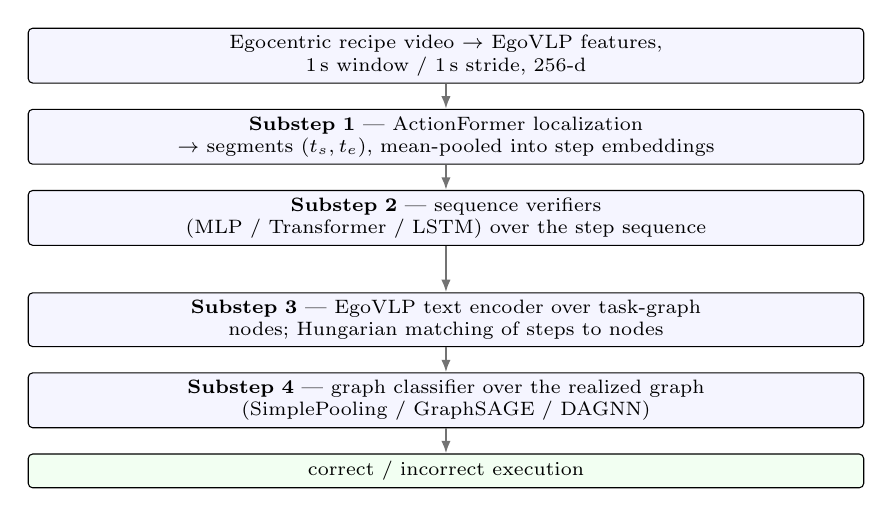
\begin{tikzpicture}[
  node distance=3.2mm,
  box/.style={draw, rounded corners=1.6pt, align=center, font=\scriptsize,
              inner sep=2.6pt, text width=0.86\linewidth, fill=blue!4},
  arr/.style={-{Latex[length=1.6mm]}, thick, draw=black!55}
]
\node[box] (v)  {Egocentric recipe video $\rightarrow$ EgoVLP features,\\1\,s window / 1\,s stride, $256$-d};
\node[box, below=of v] (s1) {\textbf{Substep 1} --- ActionFormer localization\\ $\rightarrow$ segments $(t_s, t_e)$, mean-pooled into step embeddings};
\node[box, below=of s1] (s2) {\textbf{Substep 2} --- sequence verifiers\\ (MLP / Transformer / LSTM) over the step sequence};
\node[box, below=of s1, yshift=-13mm] (s3) {\textbf{Substep 3} --- EgoVLP text encoder over task-graph\\ nodes; Hungarian matching of steps to nodes};
\node[box, below=of s3] (s4) {\textbf{Substep 4} --- graph classifier over the realized graph\\ (SimplePooling / GraphSAGE / DAGNN)};
\node[box, below=of s4, fill=green!5] (out) {correct / incorrect execution};

\draw[arr] (v) -- (s1);
\draw[arr] (s1) -- (s2);
\draw[arr] (s2) -- (s3);
\draw[arr] (s3) -- (s4);
\draw[arr] (s4) -- (out);
\end{tikzpicture}
\caption{The task-verification pipeline. Substep 2 is a graph-free control that
consumes the same step embeddings as Substep 4; the comparison between the two is
what isolates the contribution of the task graph. Everything downstream of
Substep 1 is run under \emph{two} boundary sources --- the annotations and the
trained detector --- on the same 384 recordings with the same labels.}
\label{fig:pipeline}
\end{figure}

\subsection{Step-level error recognition}

\paragraph{Baselines.} V1 pools the sub-segment features of a step with an MLP
head; V2 combines them with a Transformer encoder layer before classification. We
keep the official hyperparameters (\texttt{pos\_weight} 2.5, weight decay
$10^{-3}$, batch size 32, decision threshold 0.6 on the \emph{step} split and 0.5
on \emph{recordings}) so the comparison against the published numbers is
meaningful. As a third baseline we add a \textbf{bidirectional LSTM} (hidden 512)
over the sub-segment sequence, which the assignment suggests as a natural
alternative to attention.

\paragraph{A new backbone.} We extend the feature extraction code to
EgoVLP~\cite{lin2022egovlp}, producing $256$-d features. One implementation detail
turned out to dominate correctness: the dataloader indexes feature rows with raw
annotation timestamps \emph{in seconds}, so features must be extracted at a
1-second window and stride. Extracting at 2\,s halves the array, later steps index
past its end, and NumPy silently returns an empty $(0,256)$ slice rather than
raising. Downstream this produced a NaN loss and, at evaluation time, a fabricated
target of $0$ --- corrupting the ground truth. Three separate guards
(a NaN-skip, an \texttt{np.nan\_to\_num}, and the fabricated-target fallback) then
hid the failure and returned plausible-looking numbers. We removed all three in
favour of assertions. We note this because the symptom is instructive: with the
guards in place the pipeline reported F1 72--75 and AUC 98.9, roughly 23 points
\emph{above} the published baseline. A result that beats the reference by 23
points on the same data is a bug report, not a finding.

\subsection{Substep 1: step localization}

We train ActionFormer~\cite{zhang2022actionformer} from the CaptainCook4D fork on
our own EgoVLP features, using the official recordings split
(213 train / 62 validation / 109 test) over 353 step classes, with
\texttt{feat\_stride}$=$\texttt{num\_frames}$=30$ to match the 1\,s feature rate.
Training and inference are separated into two notebooks so the GPU job does not
re-run with every pipeline execution; the training notebook derives the final
checkpoint index from the resolved config (the fork trains for
\texttt{epochs}$+$\texttt{warmup} and names checkpoints zero-indexed) and promotes
exactly one checkpoint with a provenance record, so evaluation, exported
predictions and reported metrics cannot silently refer to different epochs.

Raw ActionFormer output is dense. We post-process with a score threshold,
class-agnostic temporal NMS and a minimum-duration filter, and we select all three
\textbf{on the validation split only}, then freeze them and score the test split
once. Each detected segment is turned into a step embedding by mean-pooling the
feature rows inside its boundaries.

Both the annotated and the predicted boundaries are exported, for all 384
recordings, as two parallel files. Every downstream substep runs on both. This is
deliberate: the annotation lists only the steps that were actually performed, so
using it as a boundary source hands the model information a detector would have to
earn.

\subsection{Substep 2: sequence verification baselines}

Three models --- MLP, Transformer and bidirectional LSTM --- consume the sequence
of step embeddings for a recording and emit one binary label. These have no access
to the task graph, and exist to answer the question the graph pipeline is
otherwise unable to answer: how much of Substep 4's performance requires a graph
at all?

\subsection{Substep 3: task-graph encoding and matching}

The 24 annotated task graphs contain 353 nodes and 369 edges in total; a linear
chain over the same nodes would have 329, so the graphs encode genuine branching
rather than a relabelled sequence. Node descriptions are encoded with the
\emph{EgoVLP text tower}, which shares an embedding space with the video tower
that produced the step embeddings. Detected steps are then matched to nodes with
the Hungarian algorithm on cosine similarity, one node per step at most.

Because the entire substep rests on the assumption that the two towers are
aligned, we measure the alignment rather than assume it (\S\ref{sec:matching}).

Matching alone discards execution order: visual features are written onto
canonical nodes and the canonical edges never change, so ``A then B'' and ``B then
A'' realize identically. Since Order Error is the largest error tag in the dataset
(795 instances), each matched node additionally carries its position in the
observed sequence, its segment boundaries, and a count of canonical edges its
position contradicts. The canonical DAG remains the structure being classified;
the observed chain is stored alongside it.

\subsection{Substep 4: classifying the realized graph}

We compare three models chosen to span a specific axis rather than to fill a
leaderboard:

\begin{itemize}
\itemsep0.15em
\item \textbf{SimplePooling} --- identical node features, \emph{no edges at all}.
The control.
\item \textbf{GraphSAGE}~\cite{hamilton2017graphsage} --- conventional
neighbourhood message passing. It is the informative choice within its family
because \texttt{SAGEConv} concatenates a node's own transformed state with the
neighbour aggregate, so a node always hears from itself and the model is not
sensitive to whether edges were symmetrised.
\item \textbf{DAGNN}~\cite{thost2021dagnn} --- topological-order processing with
attention over predecessors and a GRU update. The only model here that consumes
edge \emph{direction}.
\end{itemize}

The learnable projection the assignment asks for --- combining node text features
with matched visual features --- lives here rather than in Substep 3, because it
can only be trained where there is a loss to train it. A projector instantiated in
Substep 3 would apply a fixed random transform. It fuses the visual and text blocks
and passes the order channels through unchanged.

\subsection{Evaluation protocol}
\label{sec:protocol}

Recipe-level verification has 384 samples across 24 recipes, so protocol choices
dominate. We use \textbf{nested leave-one-recipe-out}: one recipe is held out for
test, four more are held out from the remaining 23 as an inner validation set for
epoch selection, and no metric is ever selected on the test fold. Validation is
split \emph{by recipe} rather than by recording because recordings of the same
recipe are near-duplicates; splitting by recording would place near-copies of the
validation data in training and make early stopping optimistic.

We report \textbf{pooled} metrics --- predictions from all folds concatenated and
scored once --- rather than a mean over folds. A fold contains 3--6 recordings, so
its F1 can only take a handful of discrete values, and averaging weights every
recipe equally regardless of size. Per-fold spread is kept as a dispersion
diagnostic only.

Finally, 57.29\% of recordings are labelled incorrect, so a constant ``incorrect''
predictor already scores 72.8 F1. \textbf{We read balanced accuracy and AUC}, and
every table carries the majority row.

%%%%%%%%%%%%%%%%%%%%%%%%%%%%%%%%%%%%%%%%%%%%%%%%%%%%%%%%%%%%%%%%%%%%%%%%%%%%%%%
\section{Experiments}
%%%%%%%%%%%%%%%%%%%%%%%%%%%%%%%%%%%%%%%%%%%%%%%%%%%%%%%%%%%%%%%%%%%%%%%%%%%%%%%

\subsection{Step-level error recognition}

\begin{table}[t]
\centering\small
\setlength{\tabcolsep}{4pt}
\begin{tabular}{llccc}
\toprule
Backbone & Model & Split & F1 & AUC \\
\midrule
\multirow{6}{*}{Omnivore}
 & V1 (MLP)         & step & \textbf{55.50} & \textbf{0.816} \\
 & V2 (Transformer) & step & 44.19 & 0.708 \\
 & LSTM (ours)      & step & 49.64 & 0.769 \\
 & V1 (MLP)         & rec. & \textbf{55.77} & \textbf{0.640} \\
 & V2 (Transformer) & rec. & 54.00 & 0.595 \\
 & LSTM (ours)      & rec. & 47.50 & 0.610 \\
\midrule
\multirow{2}{*}{SlowFast}
 & LSTM (ours)      & step & 51.05 & 0.683 \\
 & LSTM (ours)      & rec. & 55.53 & 0.590 \\
\midrule
\multirow{4}{*}{EgoVLP}
 & V1 (MLP)         & step & 51.13 & 0.698 \\
 & V2 (Transformer) & step & \textbf{51.44} & \textbf{0.700} \\
 & V1 (MLP)         & rec. & \textbf{55.12} & \textbf{0.631} \\
 & V2 (Transformer) & rec. & 46.74 & 0.615 \\
\bottomrule
\end{tabular}
\caption{Supervised error recognition. Omnivore and SlowFast rows are final-epoch
test metrics; EgoVLP rows are test metrics from checkpoints selected on validation
AUC. All-positive prediction scores F1 51.3 on this task, which two SlowFast
configurations fail to beat.}
\label{tab:er}
\end{table}

Table~\ref{tab:er} reports supervised error recognition.

\paragraph{The reproduction does not match the published table, and we say so.}
For Omnivore on the step split the CaptainCook4D paper reports MLP F1 24.26 and
Transformer F1 55.39; we measure 55.50 and 44.19 --- approximately the two models
exchanged. The AUCs are much closer (0.816 and 0.708 against 0.757 for both). We
report our own measurements and treat the published F1 column as not reproduced.
The likely cause is the operating point: our MLP sits at 68.64\% precision and
46.59\% recall, and a different decision threshold moves F1 a long way while
barely moving AUC.

\paragraph{Recurrence does not help.} The LSTM sits below the MLP on final-epoch
F1 on both splits and above it on best-epoch F1 on the step split. Neither ordering
is meaningful, because the Omnivore runs are not converged: omnivore/step moves
from 59.64 to 49.64 F1 between its final two epochs while its AUC moves 0.006.
Any single-epoch Omnivore F1 is a sample from a 7--10 point band. On AUC, the more
stable metric, the MLP leads on both splits, and that is the ordering we report.
With 3{,}752 training steps and features already pooled per step, there is little
sequential structure left for the LSTM to exploit.

\paragraph{SlowFast's higher F1 is a recall artefact.} It reaches the two highest
F1 scores in the table at accuracies of 47.62\% and 48.44\% --- below chance on a
34.5\%-positive task --- with recall of 87.55\% and 89.63\%. It is predicting
positive almost everywhere. Its AUC is the lowest of the three backbones.

\paragraph{EgoVLP is competitive but not better.} Our EgoVLP features reach 0.698
and 0.700 AUC on the step split against Omnivore's 0.816. This is the expected
ordering: Omnivore features were released with the dataset and extracted with the
authors' own pipeline, whereas ours are a re-implementation. What matters
downstream is not raw error-recognition accuracy but the shared video--text space,
which Omnivore does not have.

\subsection{Error recognition by category}

\begin{table}[t]
\centering\small
\setlength{\tabcolsep}{4pt}
\begin{tabular}{lrrcc}
\toprule
Category & Tags & \% pos. & F1 & AUC \\
\midrule
TechniqueError   & 502 & 7.77 & 22.45 & 0.720 \\
PreparationError & 410 & 6.14 & 19.05 & 0.757 \\
MeasurementError & 331 & 5.26 & 22.45 & 0.806 \\
TimingError      & 177 & 4.26 & 13.56 & \textbf{0.822} \\
TemperatureError &  66 & 1.00 & \textbf{0.00} & 0.739 \\
\bottomrule
\end{tabular}
\caption{Per-category error recognition, V1 (MLP) on the step split. ``\% pos.''
is the positive rate on the test split. The all-negative predictor scores F1
$=0.00$ on every row.}
\label{tab:cat}
\end{table}

Training one binary classifier per error tag (Table~\ref{tab:cat}) turns the task
from a 34.5\%-positive problem into a 1--9\%-positive one, and the consequence is
sharp. \textbf{F1 and AUC disagree, and the disagreement is the result.} Across
the twenty runs (5 categories $\times$ 2 variants $\times$ 2 splits) F1 ranges
0.00--38.27 while AUC ranges 0.578--0.916; seven of the twenty score below 25 F1
while exceeding 0.75 AUC.

TemperatureError is the cleanest case: 66 positives in 5{,}700 steps, F1 exactly
0.00 on both variants of the step split, and AUC 0.739 and 0.702. The models order
the steps correctly and never cross the decision threshold. A fixed threshold of
0.6 applied to a 1.2\%-positive task cannot do anything else.

Consequently, \textbf{ranking error types by F1 mostly ranks their base rates}. By
mean AUC the order is Timing (0.821), Temperature (0.813), Measurement (0.803),
Technique (0.668), Preparation (0.638); by mean F1 it is close to reversed. Our
pre-registered hypothesis --- that TimingError would stand out because timing
mistakes have a temporal signature that survives pooling --- is
\textbf{confirmed on AUC and refuted on F1}: first of five by AUC on only 177
tags, third of five by F1.

Two caveats we consider part of the result. Rare categories have very wide error
bars: TemperatureError has roughly 8 positive test steps, so one prediction
flipping moves F1 by several points, and no ranking here should be read as a
difficulty ordering. And Order Error, the largest tag in the dataset with 795
instances, has no per-category run at all, because ordering is not a property of a
single step. That gap is precisely what the task-graph formulation exists to
address.

\subsection{Substep 1: how good is the localizer?}
\label{sec:loc}

\begin{table}[t]
\centering\small
\setlength{\tabcolsep}{5pt}
\begin{tabular}{lrrr}
\toprule
Split & $n$ & count MAE & mean best tIoU \\
\midrule
train      & 213 & 1.92 & \textbf{0.891} \\
validation &  62 & 2.81 & 0.539 \\
test       & 109 & 3.28 & \textbf{0.520} \\
\bottomrule
\end{tabular}
\caption{ActionFormer generalization. ``count MAE'' is the mean absolute error in
the number of predicted steps; ``mean best tIoU'' averages, over annotated
segments, the tIoU of the best-overlapping prediction. Validation independently
reproduces the test figure, so the gap is generalization, not test-split
peculiarity --- note that post-processing was tuned \emph{on} validation and
validation still lands at 0.539.}
\label{tab:loc}
\end{table}

Validation mAP over the fork's 353 step classes averages 36.41\%. Post-processing
selected on validation (score $0.14$, NMS tIoU $0.20$, minimum duration $5.0$\,s)
gives, on the 109 held-out test recordings, segment-level F1 of $0.719$ at
tIoU$\geq$0.3, $0.617$ at $0.5$ and $0.411$ at $0.7$.

Table~\ref{tab:loc} is the more consequential measurement. \textbf{Boundary
quality collapses out of sample far faster than the step count does}: mean best
tIoU falls from 0.891 to 0.520, a factor of $1.7$, while count MAE degrades only
from 1.92 to 3.28. The step-count correlation with the annotation shows the same
pattern (train $0.930$, validation $0.725$, test $0.620$).

The \emph{direction} of the count error also flips. In sample the detector
over-segments (mean signed error $+1.70$); out of sample it under-segments
($-1.03$ on validation, $-1.42$ on test), with 65 of 109 test recordings
under-segmented against 31 over-segmented. This is not merely extra noise, it is a
systematic bias that reverses, and it matters in \S\ref{sec:shortcut}: an
under-segmenting detector produces realized graphs with \emph{missing nodes},
which is exactly the signal the pipeline turns out to be reading.

\subsection{Substep 2: verification without a graph}

\begin{table}[t]
\centering\small
\setlength{\tabcolsep}{5pt}
\begin{tabular}{llccc}
\toprule
Boundaries & Model & Bal. Acc & F1 & AUC \\
\midrule
\multirow{3}{*}{Annotated}
 & MLP         & 56.5 & 62.4 & 58.0 \\
 & Transformer & 58.2 & 63.6 & 59.3 \\
 & LSTM        & 58.3 & 62.6 & 59.6 \\
\midrule
\multirow{3}{*}{ActionFormer}
 & MLP         & 56.0 & 62.8 & 62.2 \\
 & Transformer & 58.4 & 63.1 & 62.6 \\
 & LSTM        & \textbf{60.9} & \textbf{64.9} & \textbf{64.1} \\
\midrule
\multicolumn{2}{l}{Majority baseline} & 50.0 & 72.8 & 50.0 \\
\bottomrule
\end{tabular}
\caption{Task verification from the step-embedding sequence alone, pooled nested
LORO over 384 recordings. Every model falls below the majority F1.}
\label{tab:sub2}
\end{table}

Table~\ref{tab:sub2} shows that verification from a flat sequence of step
embeddings barely works. All six configurations sit below the majority F1 of 72.8,
and the best AUC is 64.1. Validation loss bottoms out within the first few epochs
in most folds: these models overfit 384 recordings almost immediately.

We report this as a negative result rather than a failed experiment, because it is
the control that gives Substep 4 its meaning. Note also the direction of the
boundary effect here --- the ActionFormer rows are \emph{better}, not worse. Keep
that in mind for \S\ref{sec:sub4}.

\subsection{Substep 3: is the shared space real?}
\label{sec:matching}

Everything downstream depends on EgoVLP's video and text towers occupying the same
space, so we measure it. Over 100 recordings and 1{,}410 step pairs, video-to-text
retrieval of a step's own description reaches \textbf{26.17\% top-1 against a
7.09\% chance rate}, with correct pairs scoring $0.328$ cosine against $0.221$ for
mismatched pairs (margin $+0.107$). That is $3.7\times$ chance: real, but weak
enough to bound what the matching can contribute.

The match ratio is \emph{not} a measure of matching quality --- Hungarian pads the
cost matrix and always returns $\min(\text{steps}, \text{nodes})$ pairs --- so we
score the assignment directly. Over 5{,}358 assignments on 384 recordings,
\textbf{Hungarian assignment accuracy is 35.91\%}, against 27.12\% for
unconstrained top-1 retrieval and 7.46\% chance. The one-to-one constraint helps,
but roughly two matches in three are still wrong, and every later substep inherits
that error.

A single example makes the failure mode concrete. In recording \texttt{1\_19}, the
step \emph{``Microwave just until cheese melts''} matched the node \emph{``Continue
to Microwave for 15-30 more sec''} at $0.615$, while the exact string-to-itself
match scored only $0.521$. A wrong match outscoring an exact self-match is what
27\% top-1 looks like close up.

Finally, mean match similarity does not separate correct from incorrect executions
(0.367 vs 0.374, slightly inverted). This is expected rather than a defect:
CaptainCook4D errors are mostly wrong temperature, wrong quantity, or a skipped
step, none of which change how much a \emph{performed} step resembles its
description. The usable signal is the per-node features and the unmatched-node
mask --- a fact that will shortly become the whole story.

\subsection{Substep 4: classifying the realized graph}
\label{sec:sub4}

\begin{table}[t]
\centering\small
\setlength{\tabcolsep}{5pt}
\begin{tabular}{llccc}
\toprule
Boundaries & Model & Bal. Acc & AUC & F1 \\
\midrule
\multirow{3}{*}{Annotated}
 & SimplePooling (no edges) & 75.6 & \textbf{80.8} & 73.2 \\
 & GraphSAGE                & \textbf{75.9} & 79.6 & 73.4 \\
 & DAGNN                    & 75.4 & 79.0 & \textbf{74.2} \\
\midrule
\multirow{3}{*}{ActionFormer}
 & SimplePooling (no edges) & \textbf{65.9} & \textbf{70.6} & 67.3 \\
 & GraphSAGE                & 63.6 & 66.6 & 63.1 \\
 & DAGNN                    & 62.0 & 66.0 & 65.1 \\
\midrule
\multicolumn{2}{l}{Majority baseline} & 50.0 & 50.0 & 72.8 \\
\multicolumn{2}{l}{Hand rule: ``a step is absent''} & 79.0 & 79.1 & 73.7 \\
\bottomrule
\end{tabular}
\caption{Graph classification, pooled nested LORO over 384 recordings. The hand
rule uses no features, no training and no graph edges. The run-to-run noise floor
is $\approx$3 AUC points (\S\ref{sec:noise}).}
\label{tab:sub4}
\end{table}

Table~\ref{tab:sub4} contains the central result of this report, and it is worth
stating plainly.

\textbf{The no-edge control wins.} SimplePooling receives identical node features
and not a single edge, and it has the highest AUC under both boundary sources.
DAGNN --- the layer the assignment names for directed acyclic graphs, and the only
model here that consumes edge direction --- is the \emph{weakest} of the three.
Under annotated boundaries the spread (80.8 / 79.6 / 79.0) is inside our measured
noise floor, so the honest reading is that message passing over the task graph
contributes \emph{nothing measurable}; under predicted boundaries the no-edge
control wins by 4.0--4.6 AUC, which does clear the floor.

\textbf{A rule with no parameters matches every model.} ``Predict incorrect when a
canonical step is absent from the match'' reaches 79.1 AUC and 79.0 balanced
accuracy, above every learned model on balanced accuracy. It uses no video, no
encoder, no graph, and no training. 130 of 384 recordings are missing at least one
canonical step.

\subsection{What the graph is actually reading}
\label{sec:shortcut}

The hand rule tells us what to suspect: Hungarian matching assigns
$\min(\text{steps},\text{nodes})$ pairs, so the fraction of matched nodes is
exactly the fraction of the recipe's canonical steps that the recording contains.
CaptainCook4D's taxonomy includes a \textbf{Missing Step} tag (285 occurrences),
and recordings with such an error are structurally identifiable by counting.

This is not a train/test leak --- the feature is available at test time. It is a
shortcut created by the pipeline itself. We confirm it four ways.

\paragraph{(i) The hand rule matches the models.} As above: 79.1 AUC and 79.0
balanced accuracy with zero parameters, versus 80.8 and 75.6 for the best learned
model.

\paragraph{(ii) Masking the embeddings does not hurt.} Replacing all node features
with only the matched/unmatched mask gives 79.0 balanced accuracy and 79.1 AUC,
against 76.9 and 80.6 for the full feature set. Removing the visual and text
content entirely costs $1.5$ AUC and \emph{gains} $2.1$ balanced accuracy. Removing
the count channels instead (\emph{no\_count}) gives 75.9 / 82.1, and removing the
order channels (\emph{no\_order}) 74.4 / 81.5.

\paragraph{(iii) Swapping the boundary source collapses the graph but not the
sequence.} This is the decisive comparison, and it is only possible because
Substep 1 exports both sources for the same 384 recordings with the same labels.
Moving from annotated to predicted boundaries costs the graph models
\textbf{10.2, 13.0 and 13.0 AUC} (SimplePooling / GraphSAGE / DAGNN), while the
sequence models of Substep 2 are \emph{unaffected or slightly better}
(Table~\ref{tab:sub2}).

A sequence model never computes ``how many of the canonical steps are present'', so
it neither gains from annotated boundaries nor suffers without them. The graph
pipeline does compute it, and that is where its apparent advantage lives. The
mechanism is now measurable rather than asserted: \S\ref{sec:protocol} showed the
detector's boundary quality collapsing out of sample ($0.891 \rightarrow 0.520$)
while its step count holds up much better, and under-segmenting on held-out data.
An under-segmented recording looks, to the matcher, exactly like a recording with a
skipped step.

\paragraph{(iv) Remove the shortcut and everything collapses to chance.}
Restricting to recordings containing no Missing Step error removes the shortcut by
construction --- every remaining positive is an Order, Technique, Preparation,
Measurement, Timing or Temperature error, none of which change how many steps were
performed. On this subset the hand rule falls to chance as expected, and
\TODO{fill in from the omission-free cell: per-model AUC and balanced accuracy on
the subset, alongside each model's full-set AUC} .

\paragraph{The conclusion.} Recipe-level error detection on CaptainCook4D reduces,
in this pipeline, to \emph{``did every canonical step occur?''}. The EgoVLP
embeddings, the text encoder, the Hungarian matching and the graph structure add
little measurable beyond that, under both boundary sources and with the dataset's
true procedural topology.

\subsection{Ablations}

\paragraph{The learnable projection is worth having.} With identical folds and
seeds, replacing the fixed $0.5/0.5$ average of visual and text features with the
learnable projection the assignment specifies moves GraphSAGE from 69.03 to 76.03
balanced accuracy and 75.51 to 80.42 AUC: \textbf{$+7.00$ and $+4.91$}. Both clear
the noise floor comfortably. F1 is the more volatile column at this fold count and
should not be quoted alone.

\paragraph{Depth.} Over 2, 4, 6 and 8 layers GraphSAGE scores 81.56, 81.45, 78.27
and 73.11 AUC --- best at 2 layers and $-8.45$ by 8, consistent with over-smoothing
on graphs averaging 15 nodes. We excluded DAGNN from this study on cost grounds:
its runtime scales with (layers $\times$ topological depth), so 8 layers over
19-level graphs is 152 sequential sweeps per forward pass.

\paragraph{Edge direction.} Symmetrising the DAG's edges changes GraphSAGE by
$-1.3$ AUC (80.2 undirected vs 81.5 directed) on 30.6 versus 15.3 edges per graph.
This is the expected result for this layer specifically --- \texttt{SAGEConv}
concatenates a node's own state with the neighbour aggregate, so a node hears from
itself whether or not it has incoming edges --- which makes it a clean
\emph{control} rather than a finding: the symmetrisation choice is not quietly
driving the main table. Whether procedural order is \emph{usable} is the separate
question DAGNN answers, in Table~\ref{tab:sub4}.

\paragraph{Run-to-run noise.} \label{sec:noise}
A nine-setting sweep over learning rate and hidden size spans 5.5 AUC points
(78.0--83.5), and two runs of an identical configuration and seed have differed by
2.0 AUC, because the graph convolutions use non-deterministic CUDA scatter
operations. We therefore treat \textbf{$\approx$3 AUC points} as the floor below
which differences in this report should not be interpreted, and we say so wherever
a margin falls near it. The setting we report (lr $10^{-3}$, hidden 128) was fixed
before any test fold was scored and is not the best of the nine.

%%%%%%%%%%%%%%%%%%%%%%%%%%%%%%%%%%%%%%%%%%%%%%%%%%%%%%%%%%%%%%%%%%%%%%%%%%%%%%%
\section{Discussion and Limitations}
%%%%%%%%%%%%%%%%%%%%%%%%%%%%%%%%%%%%%%%%%%%%%%%%%%%%%%%%%%%%%%%%%%%%%%%%%%%%%%%

\paragraph{Why the graph does not help here.} We see three compounding reasons,
and they are separable. First, the matching is weak: 35.91\% assignment accuracy
means roughly two node assignments in three are wrong, so the features written onto
the graph are largely misplaced. Second, the graphs are small --- 353 nodes over 24
recipes, about 15 nodes and 15 edges each --- so there is little topology for
message passing to exploit, and two layers already cover most of a graph's
diameter. Third, and most fundamentally, the label is dominated by an error type
(Missing Step) that is fully determined by node presence, which a pooling model
reads directly without needing edges at all.

\paragraph{This is a property of the pipeline, not a claim about task graphs.}
We do not conclude that procedural structure is uninformative. We conclude that
\emph{this} pipeline, on \emph{this} dataset, extracts almost all of its signal
from step presence. A stronger matcher, or a label distribution not dominated by
omissions, could well change the answer --- and our order-violation statistics
suggest the raw material is there: 39.3\% of realized edges are violated under
annotated boundaries, and 98.4\% of recordings violate at least one.

\paragraph{Limitations.} (a) The omission-free confirmation is run on a subset with
fewer recipes, so its folds are smaller and noisier than the main table's.
(b) All recipe-level numbers rest on 384 samples with a 3-point noise floor;
differences we call real clear it, but not by large margins. (c) Our EgoVLP
features are a re-implementation, and their step-level error-recognition AUC sits
below the released Omnivore features; a better egocentric video--text model would
raise the matching accuracy that bounds Substep 3. (d) We report a single seed per
configuration for the main table, with repeated runs used only to measure the noise
floor.

%%%%%%%%%%%%%%%%%%%%%%%%%%%%%%%%%%%%%%%%%%%%%%%%%%%%%%%%%%%%%%%%%%%%%%%%%%%%%%%
\section{Conclusion}
%%%%%%%%%%%%%%%%%%%%%%%%%%%%%%%%%%%%%%%%%%%%%%%%%%%%%%%%%%%%%%%%%%%%%%%%%%%%%%%

We built the full task-verification pipeline for CaptainCook4D --- ActionFormer
localization on our own EgoVLP features, sequence baselines, EgoVLP-text task-graph
encoding with Hungarian matching, and a graph classifier --- and evaluated it under
a protocol that selects nothing on the test fold, alongside step-level error
recognition baselines including a per-category analysis.

The result we consider most valuable is the one that took the most work to
establish: on this benchmark, a graph classifier that reaches 80.8\% AUC is mostly
counting steps. A no-edge control is the strongest model, DAGNN is the weakest, and
a zero-parameter rule matches both. We reached that conclusion through four
independent experiments rather than one, and we quantified the mechanism by
measuring how the detector's boundary quality and step count degrade at different
rates out of sample.

The methodological point generalises beyond this dataset. Every substep of this
project contained at least one defect of the same shape --- a silent fallback that
turned a failure into a plausible number, or a selection step that peeked at data
it should not have seen. Empty feature slices became fabricated labels; missing
segments became one segment spanning the video; training-loss selection picked the
most overfit checkpoint; test-set selection picked the luckiest epoch. None of them
were loud. The fix, in every case, was to make them loud --- and the no-edge
control and the hand rule are the same idea applied to the model itself.

{\small
\bibliographystyle{ieeenat_fullname}
\bibliography{main}
}

\end{document}
